\documentclass{beamer}
\usepackage[T1]{fontenc}
\usepackage[utf8]{inputenc}
\usepackage{lmodern}
\usepackage[brazil]{babel}
\usepackage[labelformat=empty]{caption}
\usepackage{graphicx}
\usetheme{Luebeck}
\title[Padrão Model-View-Controller]{Padrão Model-View-Controller}
\author{Ana Luísa Losnak. Luiz Armesto. Renan Fichberg.}
\date{Novembro 4, 2014}
\institute{Instituto de Matemática e Estatística da Universidade de São Paulo (IME-USP)}
\begin{document}

\begin{frame}
\titlepage
\end{frame}

\begin{frame}
\frametitle{Introdução}
\begin{itemize}
	\item O que é um padrão?
	\item O padrão MVC
	\item Alguns padrões similares ao MVC
\end{itemize}
\end{frame}

%TODO: o que é um padrão (não há necessidade de dar exemplos. O tema por si só já é um exemplo)
\begin{frame}
\frametitle{O que é um padrão?}
	Em Engenharia de Software, um padrão de design é uma solução geral que pode ser reutilizada para resolver um problema recorrente de um contexto específico de Design de Software.
\end{frame}

%TODO: O padrão MVC
\begin{frame}
\frametitle{O padrão MVC}
\begin{itemize}
	\item Surgimento
	\item Por que usar?
	\item O padrão MVC
\end{itemize}
\end{frame}

\begin{frame}
\frametitle{O padrão MVC}
\framesubtitle{Surgimento}
	O cientista da computação norueguês Trygve Reenskaug inicialmente introduziu o padrão MVC no Smalltalk-76 enquanto visitava a Xerox Parc, nos anos 70. Na decada posterior, Jim Althoff e outras pessoas implementaram uma versão do padrão para a biblioteca do Smalltalk-80. A partir de então, nos anos seguintes o padrão evoluiu o suficiente para que surgisse variantes, como o HMVC (\textit{Hierarchical Model-View-Controller}), o MVA (\textit{Model-View-Adapter}) e o MVP (\textit{Model-View-Presenter}).
\end{frame}

\begin{frame}
\frametitle{O padrão MVC}
\framesubtitle{Por que usar?}
\begin{itemize}
	\item Interfaces de usuário estão propensas a mudar freqüentemente e, portanto, isto não pode ser uma tarefa complicada
	\item Ganhar flexibilidade: reduzir o entrelaçamento da interface de usuário com o núcleo funcional.
	\item Diminuir custos e propensão a erros na construção do sistema
\end{itemize}
\end{frame}

\begin{frame}
\frametitle{O padrão MVC}
\framesubtitle{}
	O padrão de arquitetura divide uma aplicação em três componentes que estão interconectados: o model, as views e os controllers, sendo os últimos dois os componentes que compreendem a interface de usuário.
\begin{center}
	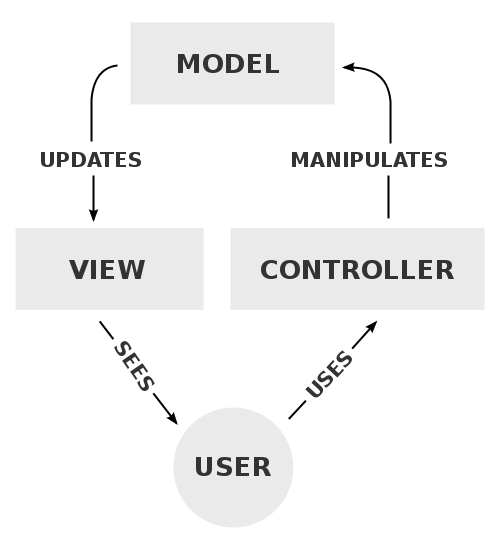
\includegraphics[scale=0.2]{MVC.jpg}
\end{center}
\begin{center}
	\tiny{\textit{Fonte: wikipedia}}
\end{center}
\end{frame}

\begin{frame}
\frametitle{O padrão MVC}
\framesubtitle{A tríade: os três componentes do MVC}
\begin{itemize}
	\item Model: encapsula os dados e a funcionalidade. É independente de representações específicas das saídas de dados e do comportamento da entrada de dados.
	\item View: apresenta as informações para o usuário. Os dados apresentados são obtidos do model. Podem haver diversas views para o model.
	\item Controller: cada view tem um controller associado à ela. Controllers recebem eventos de entrada, como click de mouse ou leitura de teclado. Tais eventos são então traduzidos em requisições para o model ou para a view. É pelo controller que o usuário interage com o sistema.
\end{itemize}
\end{frame}

\begin{frame}
\frametitle{Softwares que utilizam o MVC}
\framesubtitle{}
\end{frame}

\begin{frame}
\frametitle{Softwares que utilizam o MVC}
\framesubtitle{Rails não é MVC!}
	Apesar do que se diz por aí, o famoso framework \textit{Rails} não é MVC, mas sim um modelo similar a este, chamado \textbf{Model 2}. Por que?\\
\end{frame}

\begin{frame}
\frametitle{Softwares que utilizam o MVC}
\framesubtitle{Rails não é MVC!}
	No MVC clássico, um model pode notificar as views a respeito das mudanças que aconteceram (a partir do padrão \textit{Observer}). No Rails
	nós não notificamos as views a partir do model, o controller simplesmente passa o dado do model para as views e se encarrega da geração do HTML que 
	é posteriormente enviado ao browser, como exibido no esquema abaixo:
	\begin{center}
		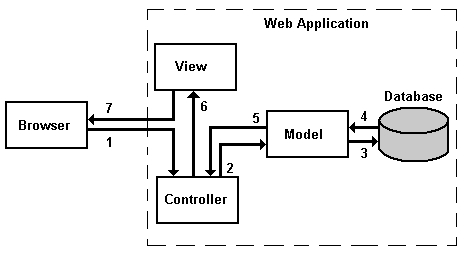
\includegraphics[scale=0.4]{RailsMVC.jpg}
	\end{center} 
\end{frame}

\begin{frame}
\frametitle{Alguns padrões similares ao MVC}
\framesubtitle{O Model 2}
	A seguir, um diagrama do \textit{Design Pattern} \textbf{Model 2}, usado no framework \textit{Rails}, mencionado no último slide.\\
	\begin{center}
		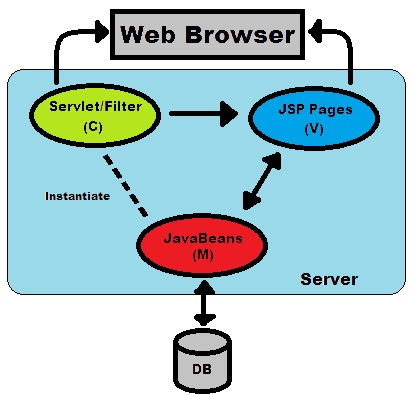
\includegraphics[scale=0.2]{Model2.jpg}
	\end{center}
	\begin{center}
		\tiny{\textit{Fonte: wikipedia}}
	\end{center} 
\end{frame}

\begin{frame}
\frametitle{Alguns padrões similares ao MVC}
\framesubtitle{O Hierarchical Model–View–Controller (HMVC)}
	O \textbf{HMVC} é uma variação do MVC, similar a um outro chamado \textit{Presentation–Abstraction–Control (PAC)}, que surgiu como uma resposta aos problemas
	relacionados a escalabilidade.
	%inserir uma imagem da arquitetura do HMVC aqui 
\end{frame}

\begin{frame}
\frametitle{Alguns padrões similares ao MVC}
\framesubtitle{O Movel-View-Adapter (MVA)}
	Uma outra variação do MVC é o \textbf{Model-View-Adapter (MVA)}, que traz com ele uma diferença de estilo:\\
	Não há comunicação direta entre a View e o Model.
	%inserir uma imagem de MVA
	%https://www.palantir.com/2009/04/model-view-adapter/
\end{frame}

\begin{frame}
\frametitle{Alguns padrões similares ao MVC}
\framesubtitle{O Movel-View-Presenter (MVP)}
	Nesta outra variação do MVC, nomeada \textbf{Model-View-Presenter (MVP)}, a View é a responsável por manipular os eventos da interface de usuário, função do controller no MVC tradicional.
	%inserir uma imagem de MVP
\end{frame}

\begin{frame}
\frametitle{Padrões similares ao MVC}
\framesubtitle{Comparações entre os modelos apresentados}
	%inserir uma imagem com os modelos lado a lado.
\end{frame}

\end{document}
